\chapter{Resultados}
\label{resultados}

\section{Modelo}
\todo[inline]{print do código no tema claro, com huperparâmetros}

Abaixo encontra-se o código em Python da implementação de um módulo LSTM por meio do Pytorch.

\begin{figure}[ht]
    \centering
    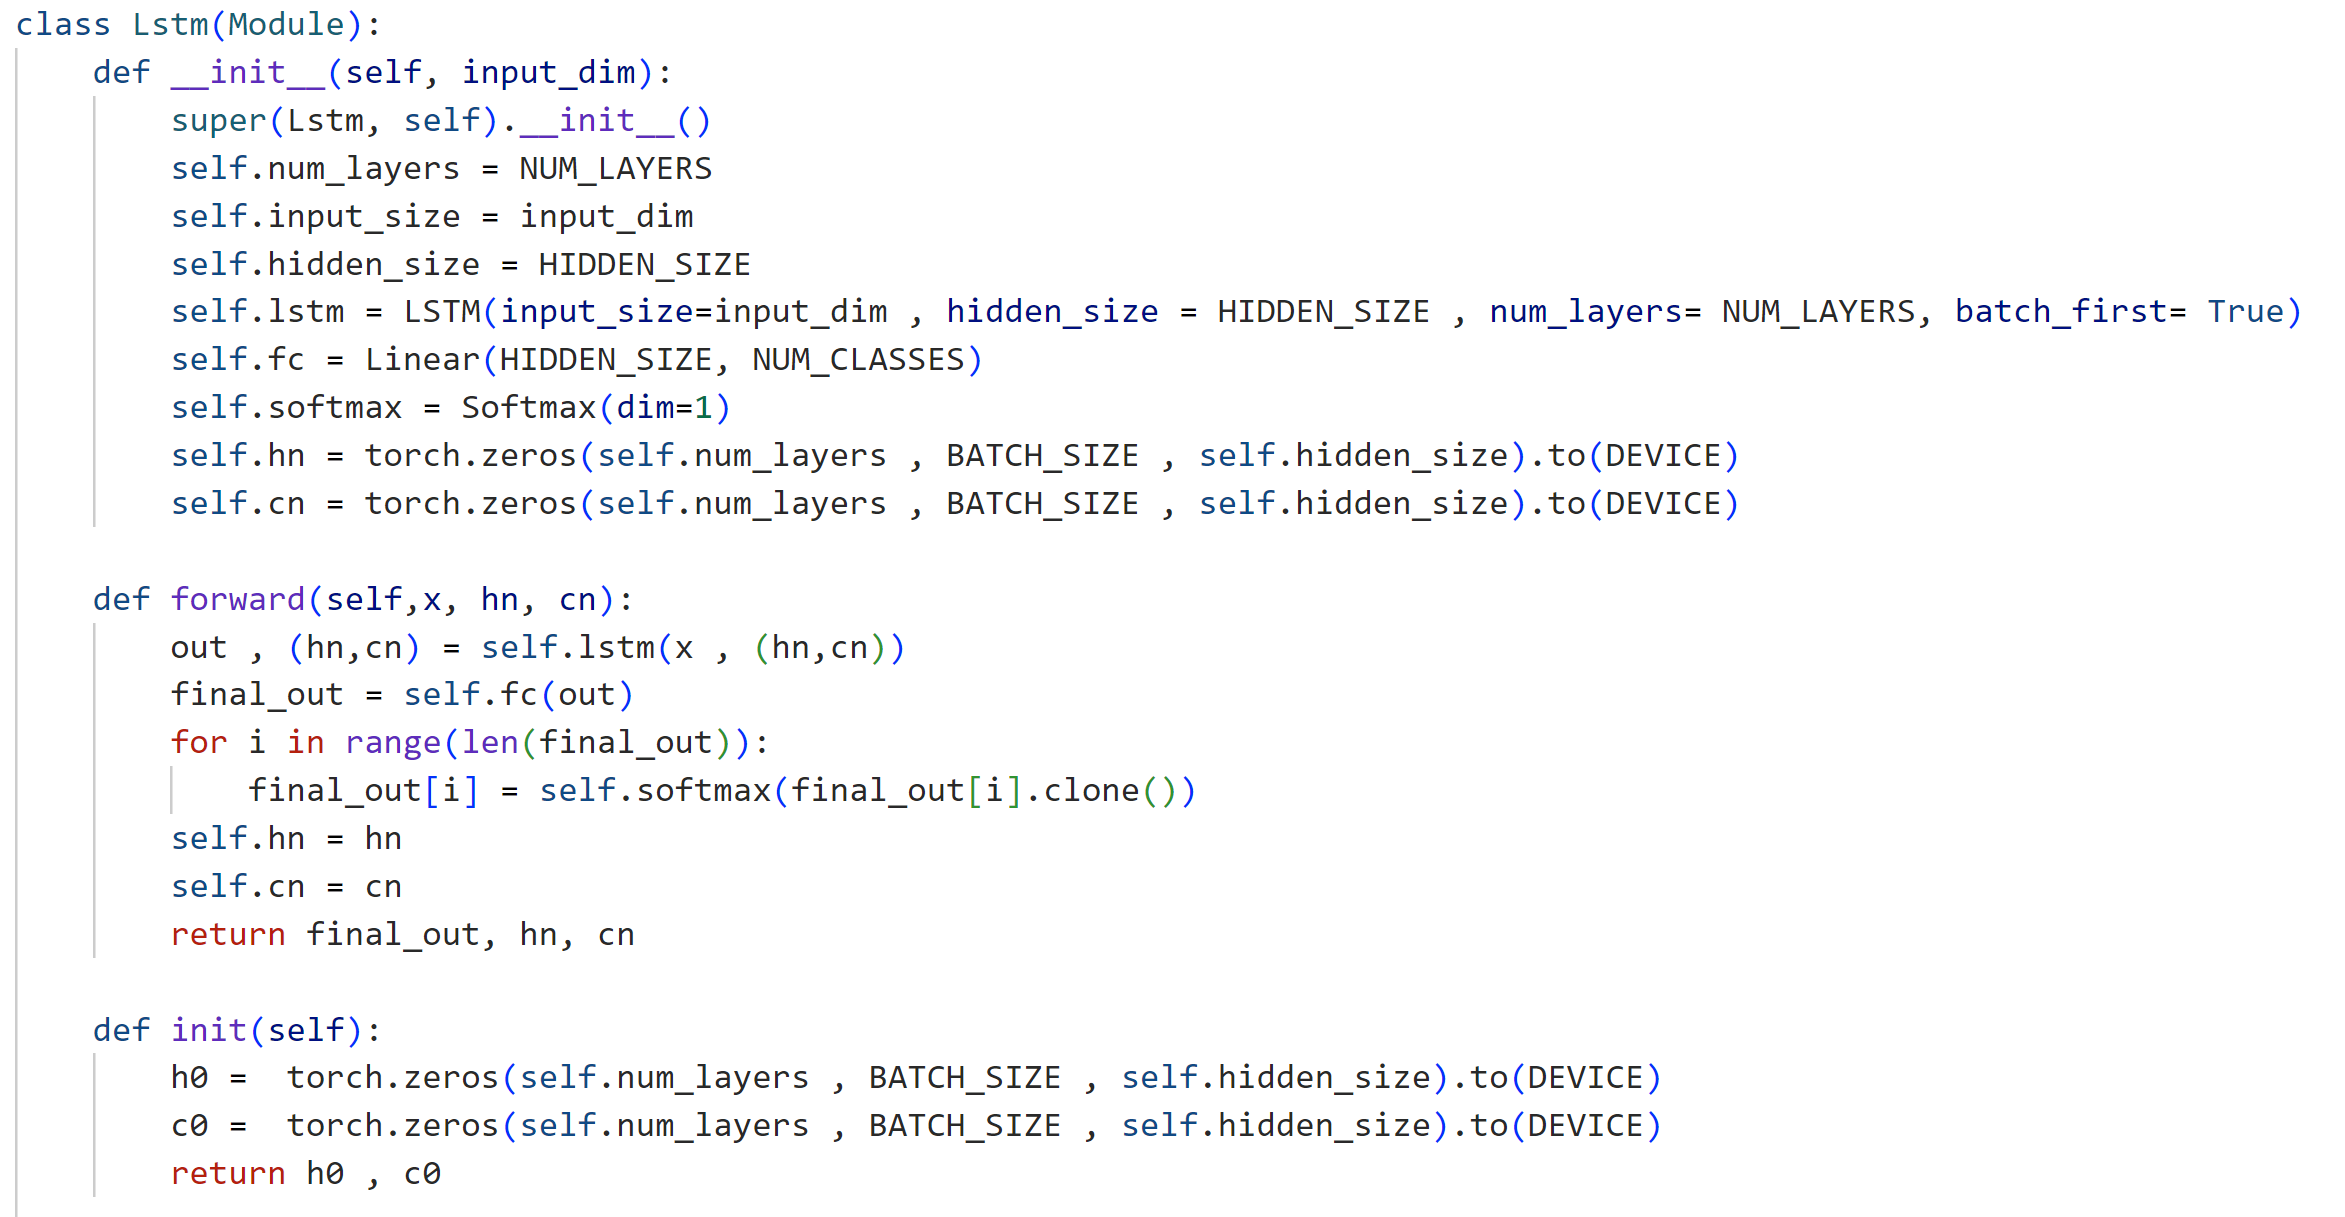
\includegraphics[scale=0.5]{tg1/figuras/codigo.png}
    \caption{Código do modelo LSTM}
    \label{fig:codigo_lstm}
\end{figure}

Os hiperparâmetros são:
\begin{table}[h]
    \centering
    \begin{tabular}{|l|c|l|}
        \hline
        \textbf{Parâmetros} & \textbf{Significado} & \textbf{Valor} \\
        \hline
        NUM\_LAYERS & Número de camadas & 2 \\
        input\_dim & Dimensão da entrada (número de features) &  68\\
        HIDDEN\_SIZE & Tamanho do estado oculto &  60\\
        \hline
    \end{tabular}
    \caption{Parâmetros do Modelo}
    \label{tab:hiperparametros}
\end{table}

Abaixo encontra-se o código do algoritmo de \textit{loss} implementada via Pytorch \cite{Lin_Goyal_Girshick_He_Dollar_2017}.

\begin{figure}[ht]
    \centering
    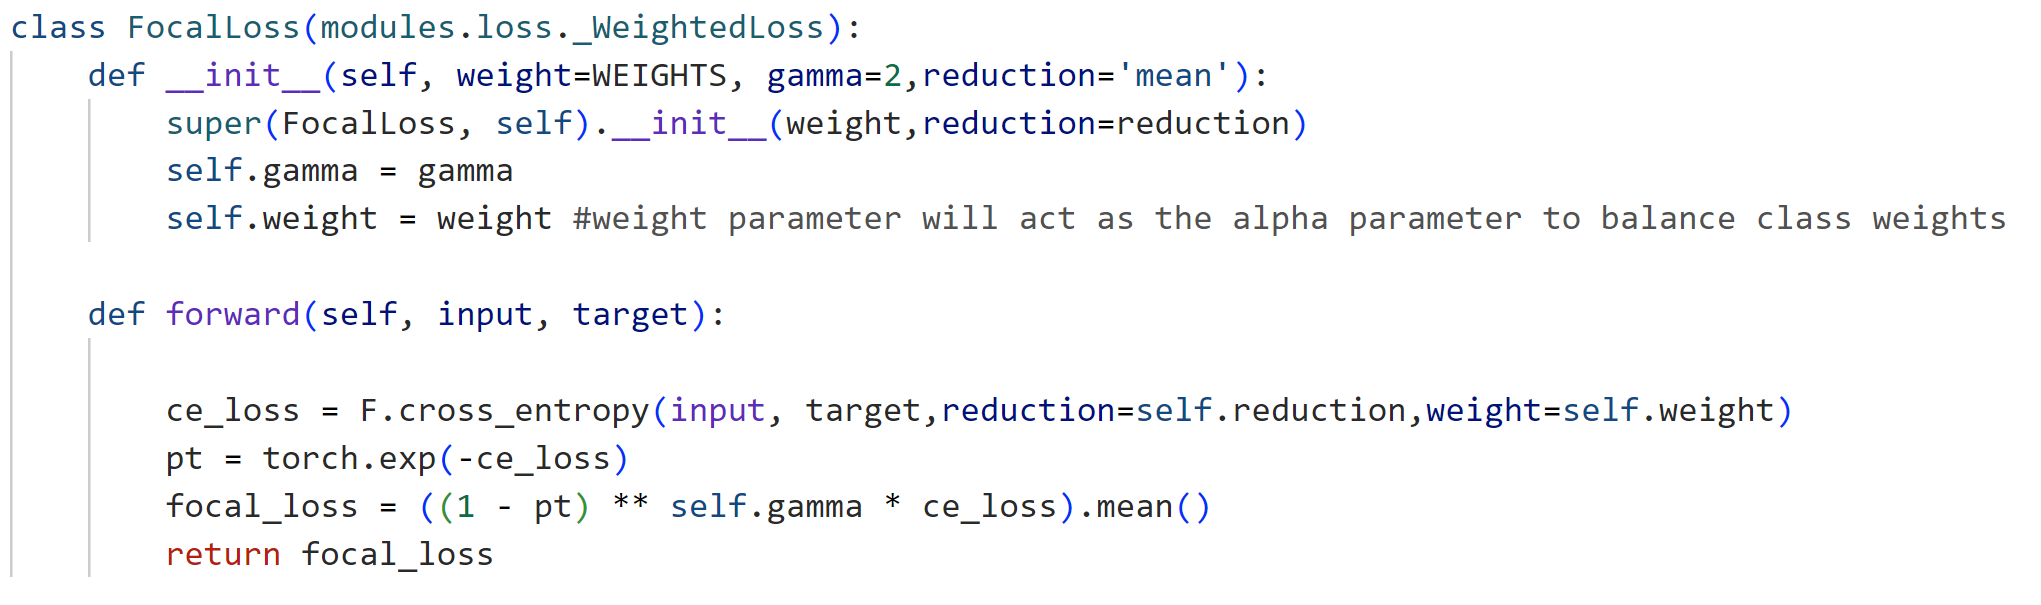
\includegraphics[scale=0.5]{tg1/figuras/loss.png}
    \caption{Código do modelo de Loss Focal}
    \label{fig:loss}
\end{figure}

\section{Metodologia}


%Por meio da biblioteca scikit-learn, é possível escrever um código simples que emprega o uso do modelo Random %Forest e com fácil customização. 

Podemos descrever o funcionamento do códigos de treinamento dos modelos por meio do seguinte fluxograma, na figura \ref{fig:rfflux}:

\begin{figure}[H]
	\centering
	\begin{minipage}{0.98\linewidth}
		\centering
		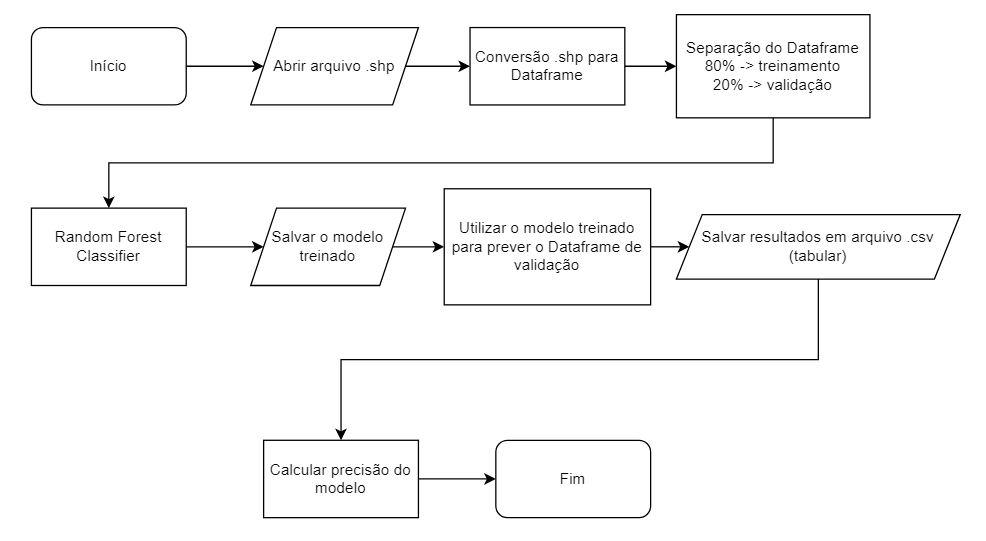
\includegraphics[width=\linewidth]{tg1/figuras/rfflux.png}
		\caption{Fluxograma do funcionamento do código do Random Forest} \label{fig:rfflux}
	\end{minipage}
\end{figure}
\todo{fluxograma do LSTM!!!}
Os parâmetros utilizados para a função do \textit{Random Forest Classifier} foram os valores padrões utilizados pelo scikit-learn \cite{sklearnrfc}, com o objetivo de obter-se um primeiro resultado para o nosso modelo. Enquanto os parâmetros do MLP foram sendo definidos até que a rede apresentasse \textit{overfitting}, demonstrando capacidade de generalização. Após isto, os seus hiper-parâmetros foram ajustados até fossem atingidos os melhores resultados encontrados.

\subsection{Lidando com Overfitting}
O problema de overfitting foi encontrado durante alguns testes como consequência do mal balanceamento do dataset. A classe 3, referente às queimadas de sub-bosque, representa 1.8\% do dataset, o que resulta em 0\% de acurácia para esta classe para um modelo treinando sem qualquer algoritmo de balanceamento.

É comum na literatura encontrar exemplos de "data augmentation" \cite{survey_data_augmentation}. Trata-se de algoritmos capaz de expandir um dataset sem comprometer de forma significativa seu valor como dado de treinamento. Neste trabalho, optou-se por empregar uma redução de dados como estratégia de balanceamento. Esta estratégia envolve eliminar de forma aleatória dados de rótulos diferentes de forma a se aumentar a representação do tipo de dados de menor presença no dataset. Este tipo de estratégia acabou resultando em overfitting, conforme a imagem a seguir.

\begin{figure}[ht]
    \centering
    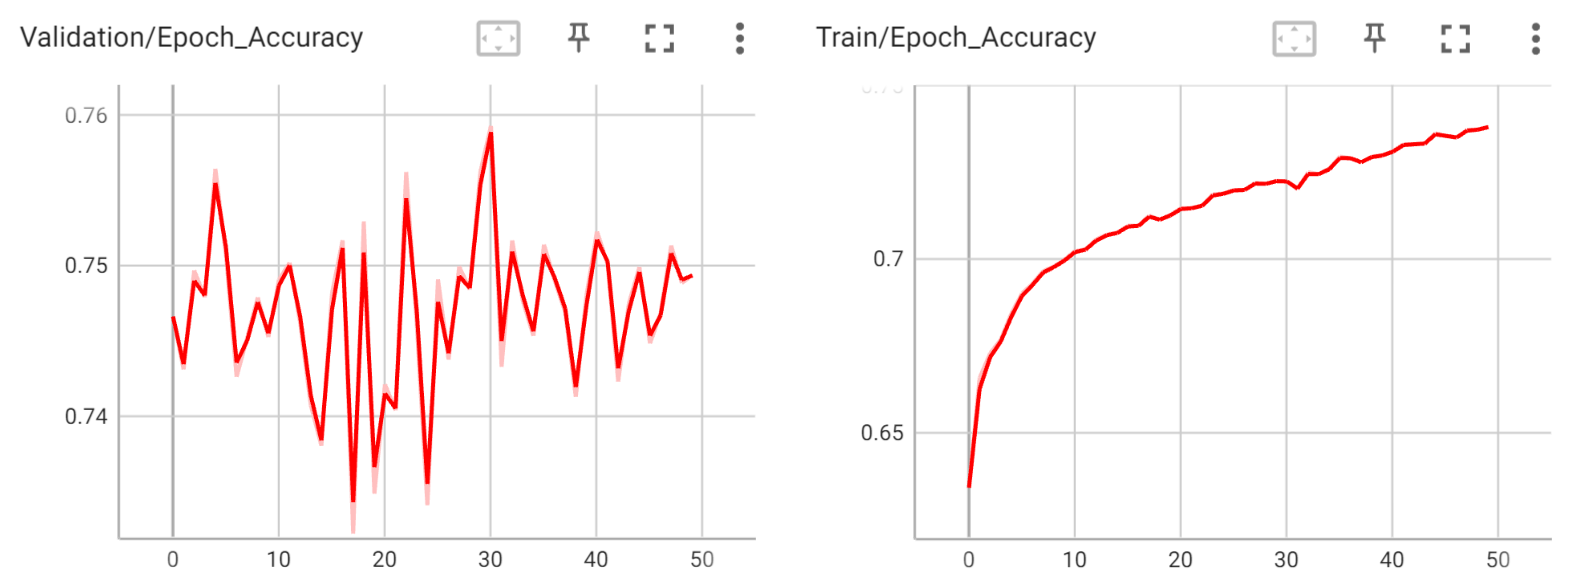
\includegraphics[scale=0.5]{tg1/figuras/overfit.png}
    \caption{Overfitting no treinamento}
    \label{fig:overfitting}
\end{figure}

Na figura \ref{fig:overfitting} pode-se ver que embora a acurácia de treinamento esteja aumentando, a acurácia de validação não está melhorando. Dessa forma, pode-se dizer que a rede está se tornando "viciada" nos dados de treinamento e aprendendo a interpretá-los bem mas não está aprendendo a interpretar dados estranhos.

Tendo em mãos estes resultados, optou-se por utilizar um leve balanceamento, aumentando a representatividade de 1.8\% para 5\%. Esta proporção foi obtida de forma empirica como um valor que representa uma melhora significativa na acurácia para a classe 3 porém sem reduzir demais a acurácia para as demais classes.


\subsection{Organização em Série Temporal}

Transformar os dados existentes em uma série temporal envolve a adição de uma nova dimensão, a temporal. Em termos práticos, isto é efetuado por meio de uma dimensão acrescentada aos tensores dos dados transformando eventos discretos em dados sequenciais. 

Os dados disponibilizados pelo CENSIPAM possuem identificadores rotulados como "id\_evento". Estes códigos agrupam diferentes detecções de incêndios como pertencentes a um mesmo foco de incêndio e é necessário para a transformação dos dados em uma série temporal. Em outras palavras, cada dados possui três dimensões: o ID representando o foco de incêndio, a quantidade de detecções relativas a este mesmo incêndio, e todos os dados de cada uma destas detecções.

No entanto, esta abordagem envolve o desafio de transformar estes dados em tensores. Todo o código utilizado é construído a partir do Pytorch \cite{NEURIPS2019_9015}, que utiliza tensores como tipo de dado. Tensores são matrizes multi-dimensionais, apenas uma forma de se organizar dados de forma lógica. Por exemplo, pode-se imaginar um tensor tridimensional como um cubo, tratando-se de um tensor cujo as três dimensões são iguais.

Em outras palavras, tensores são uma forma de se estruturar dados de forma regular, onde cada amostra de dados possui dimensões constantes e condizentes com as dimensões do tensor. No entanto, os dados em questão não são regulares pois são obtidos a partir de fenômenos aleatórios e caóticos, de queimadas sobre um território florestal de proporções continentais. Por isso é necessário o emprego de alguma técnica de tratamento de dados que possa regularizá-los, permitindo sua manipulação como tensores.

\subsubsection{Padding}

O desafio em questão é transformar dados de comprimento variado em dados padronizados com o mesmo comprimento, para que possam ser organizados como um tensor tridimensional. Dessarte, é necessário de se empregar um algoritmo capaz de preencher lacunas e eliminar excessos para garantir que todos os dados tenham as mesmas proporções.

"\textit{Padding}" não se trata de um algoritmo específico, mas de qualquer algoritmo capaz de preencher lacunas para garantir regularidade entre dados. Tratando-se de séries temporais, os algoritmos de \textit{Padding} mais comuns envolvem preencher com zeros, com médias ou repetindo valores. Neste trabalho, optou-se por preencher as lacunas repetindo-se a última detecção do evento e eliminando as primeiras em casos de eventos muito grandes. 

\begin{figure}[ht]
    \centering
    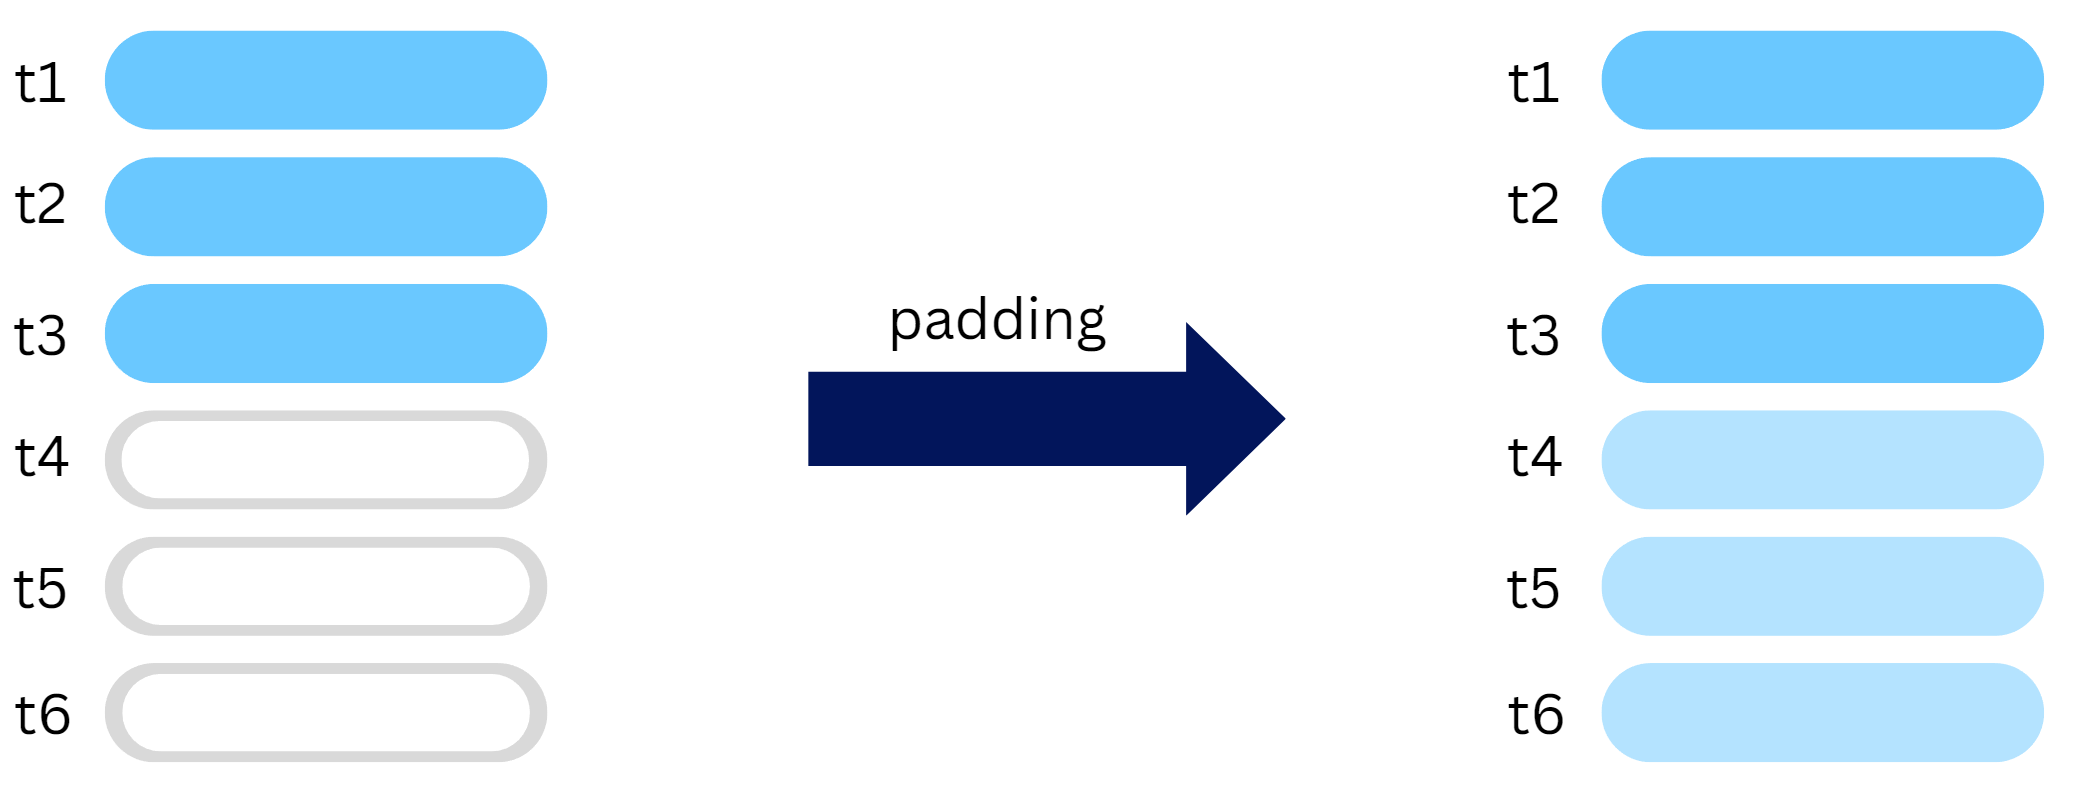
\includegraphics[scale=0.5]{tg1/figuras/padding.png}
    \caption{Representação de Padding}
    \label{fig:padding}
\end{figure}


O motivo para esta escolha é dado pela observação do comportamento da saída da rede ao longo de cada passagem pelos dados. Observou-se que a rede tende ajustar sua saída rapidamente, dentro de 5 iterações, e a manter esta saída até o final, revelando que converge em um valor rapidamente. Logo, foram evitados algoritmos que causem ruído no início da série temporal, período de maior convergência do algoritmo.


\subsection{Servidores do Censipam}

A parceria com o CENSIPAM se deu com o intuito de integrar o modelo de aprendizado como uma ferramenta classificadora em seu sistema. Para isto, foi-se fornecido acesso a uma máquina por meio de tunelamento SSH para que o projeto tenha acesso ao banco de  dados em tempo real.

Dessa forma, o código foi implementado no sistema para que rode continuamente. Atualmente, o programa aguarda até as 23 horas de cada dia para iniciar seu processamento. Neste momento, são requisitados os dados novos, referentes ao dia atual, e os dados antigos de mesmo ID, com apenas XXX features. A partir delas, o algoritmo de adição de features adiciona as demais. Em sequência, os dados passam pela etapa de pré-processamento, sendo normalizados e efetuado o padding. Por fim, o algoritmo de aprendizado de máquina classifica estes dados e monta arquivos dos tipos CSV e SHP com todos os dados classificados.

\subsection{Dados de Treinamento e Dados em Produção}
\todo[inline]{mostrar gráficos comparando ambos datasets}
Os fornecidos para o treinamento do algoritmo e os dados obtidos em produção nos servidores são diferentes. Primeiramente, os dados de treinamento vão até o ano 2022 enquanto os dados disponíveis nos servidores se iniciam em 2023. Além disso, é interessante de se estudar a continuidade entre estes dados, de forma a garantir que sua qualidade é similar à dos dados utilizados no treinamento, ou se houve alguma mudança na forma como são produzidos, como por exemplo, mudança de métrica de metros para quilômetros.


\subsection{Treinamento x Produção}
\subsection{}

\section{Métricas de Avaliação do Modelo}

A avaliação de modelos de aprendizado de máquina é crucial para desenvolver um bom algoritmo de aprendizado de máquina. Métricas de avaliação fornecem uma medida objetiva do desempenho do modelo, permitindo comparações entre diferentes abordagens.

No algoritmo de treinamento do modelo, separou-se o dataset entre validação e treinamento, sendo 80\% destinado para o treinamento e 20\% para a validação, separados cronologicamente. As métricas são obtidas de época em época e podem ser observadas por meio do módulo Tensorboard, disponível pelo Tensorflow \cite{tensorflow2015-whitepaper}, ou pelo terminal do programa como uma tabela ao finalizar-se o treinamento.

Métricas são essenciais no ajuste fino dos hiper parâmetros do modelo de aprendizado de máquina. A partir deles, é possível diagnosticar problemas como \textit{overfitting} ou explosão de gradiente. Os dados gerados são acurácia, precisão, \textit{recall} e \textit{f-score} para cada classe e no total de forma ponderada. Além disso também são registrados os valores dos pesos dos nós da rede neural de forma a se observar explosões ou desaparecimentos de gradiente.

\begin{figure}[ht]
    \[F_{1} = \frac{2tp}{2tp + fp + fn}\]
    \caption{Fórmula para \textit{F-score}}
\end{figure}

\begin{figure}[ht]
    \[ \textit{recall} =  \frac{tp}{tp + fn}\]
    \caption{Fórmula para \textit{recall}}
\end{figure}

Onde "tp" é quantidade de verdadeiros positivos, "fp" falsos positivos e "fn" falsos negativos. \textit{F-score} é uma métrica útil para medir o aprendizado da rede pois é uma forma de levar em consideração o desequilíbrio entre classes. Por exemplo, em uma tarefa de classificação cujo a classe 1 representa apenas 1\% dos dados teria uma acurácia de 99\% caso exibisse apenas a classe 0 como resultado, porém o \textit{F-score} traria um resultado péssimo, informando a falha da rede. Já o \textit{recall}, que é utilizado no cálculo do \textit{F-score}, mede a capacidade de um modelo identificar corretamente todos os exemplos positivos em um conjunto de dados. 

\todo[inline]{inserir tabela com performance e prints do tensorboard}

    
\begin{table}[h]
    \centering
    \begin{tabular}{|c|c|c|c|c|}
        \hline
        & Acurácia & Precisão & Recall & F1-Score \\
        \hline
        classe 1 & 0.795 & 0.904 & 0.795 & 0.846 \\
        classe 2 & 0.804 & 0.772 & 0.804 & 0.788 \\
        classe 3 & 0.290 & 0.237 & 0.289 & 0.261 \\
        classe 4 & 0.620 & 0.485 & 0.619 & 0.544 \\
        \hline
        Ponderada & 0.767 & 0.786 & 0.767 & 0.774 \\
        \hline
    \end{tabular}


    \vspace{10pt}
    
    \begin{tabular}{|c|c|}
        \hline
        Classe & Quantidade \\
        \hline
        classe 1 & 73647 \\
        classe 2 & 64205 \\
        classe 3 & 3136 \\
        classe 4 & 19986 \\
        \hline
    \end{tabular}
    \caption{Resultados da Avaliação}
    \label{tab:resultados}
\end{table}

% \section{Evolução do modelo MLP}

% DROP OUT, NORM BATCH, LAYERS, BATCH SIZE, TREINAMENTO, MAQUINA UTILIZADA, ETC

% \section{Análise de Resultados}

% Na última etapa de calculo da precisão do modelo Random Forest, foi obtido os valores da tabela \ref{tab:rf} para quando classificamos o \textit{dataframe} de validação.

% \begin{table}[H]
% \caption{Precisão do modelo Random Forest}
% \label{tab:rf}
% \begin{tabular}{lllll}

%                  & Precision & Recall & F1-score & Quantidade \\
% 0                & 1.00      & 1.00   & 1.00     & 124125  \\
% 1                & 1.00      & 1.00   & 1.00     & 29652   \\
% 2                & 0.84      & 0.73   & 0.78     & 1866    \\
% 3                & 0.86      & 0.92   & 0.89     & 3615    \\
% Acurácia         &           &        & 0.99     & 159258  \\
% Média aritmética & 0.92      & 0.91   & 0.92     & 159258  \\
% Média ponderada  & 0.99      & 0.99   & 0.99     & 159258 
% \end{tabular}
% \end{table}


% A partir do resultado salvo em arquivo .csv, também é possível criarmos uma matriz de confusão para visualizarmos o comportamento da rede, conforme temos na figura \ref{fig:mcrf}. Quantos valores de cada tipo de fogo ela foi capaz de prever corretamente, e quantos ela errou, e para quais valores.

% \begin{figure}[htb]
% 	\centering
% 	\begin{minipage}{0.98\linewidth}
% 		\centering
% 		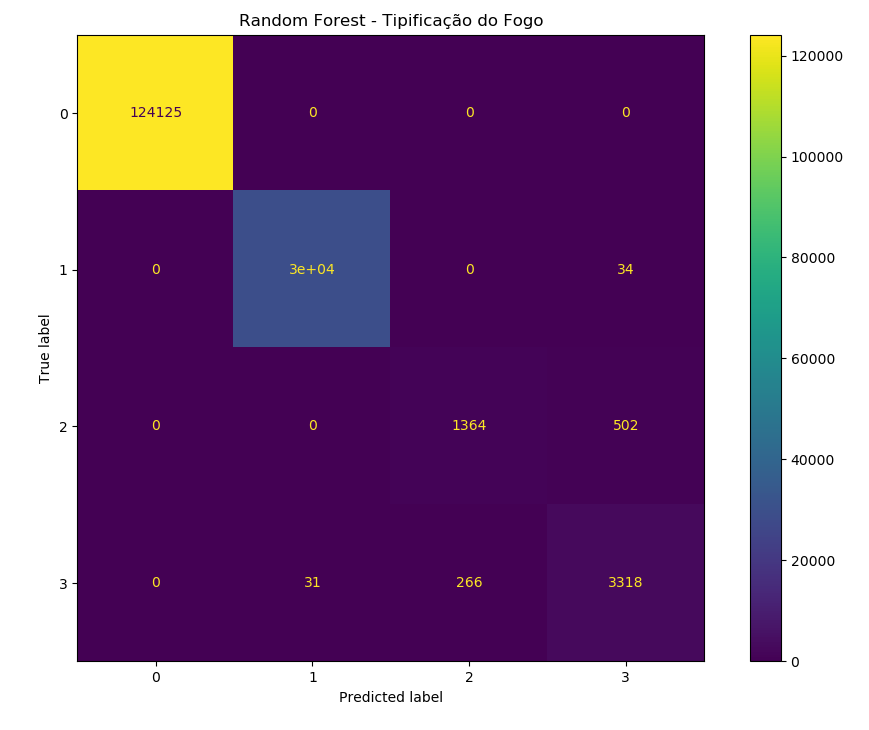
\includegraphics[width=\linewidth]{tg1/figuras/matrizconfusaorandomforest.png}
% 		\caption{Matriz de confusão para Random Forest} \label{fig:mcrf}
% 	\end{minipage}
% \end{figure}

% %\todo{COLOCAR METRICAS DO MLP}

% \begin{table}[H]
% \caption{Precisão do modelo MLP}
% \label{tab:rf}
% \begin{tabular}{lllll}

%                  & Precision & Recall & F1-score & Quantidade \\
% 0                & 1.00      & 1.00   & 1.00     & 124125  \\
% 1                & 0.98      & 1.00   & 0.99     & 29652   \\
% 2                & 0.69      & 0.66   & 0.68     & 1866    \\
% 3                & 0.79      & 0.84   & 0.81     & 3615    \\
% Acurácia         &           &        & ??     & 159258  \\
% Média aritmética & ??      & ??   & ??     & 159258  \\
% Média ponderada  & 0.99      & 0.99   & 0.99     & 159258 
% \end{tabular}
% \end{table}

